% Figure 2 - scatter F1 x distancia (Secao 6.1).
% Gerada por 03_analysis/11_fig2_scatter_flow_distance.py.

\begin{figure}[t]
\centering
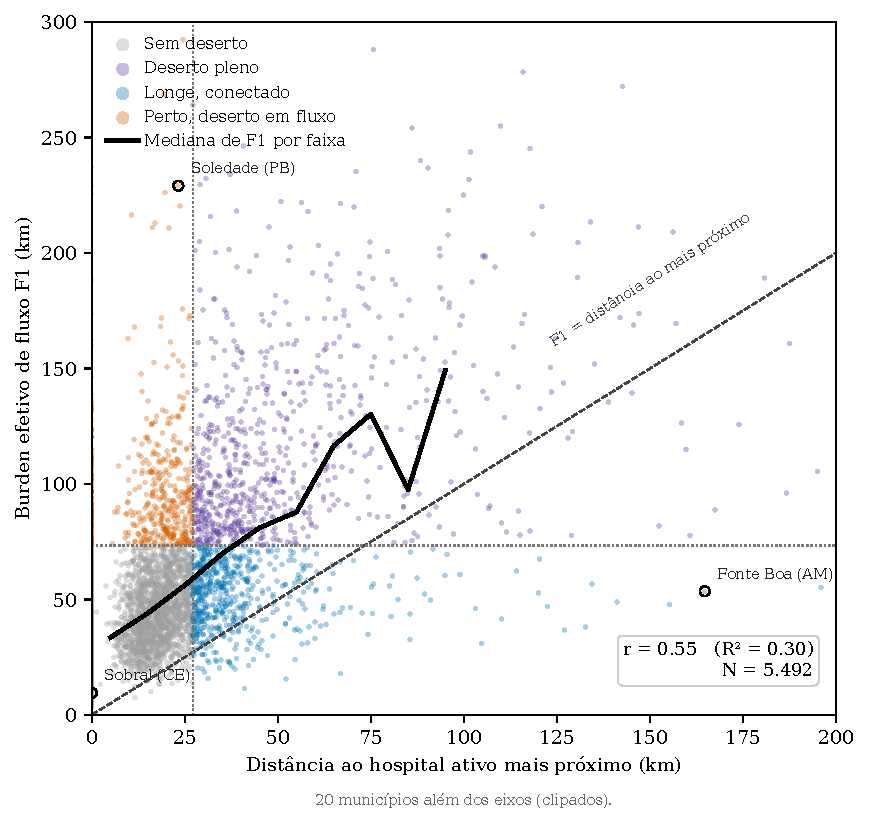
\includegraphics[width=0.82\linewidth]{../04_figures/fig2_scatter.pdf}
\caption{\textbf{Fluxo e distância são correlacionados, mas não intercambiáveis.}
Cada ponto é um município ($N=5.492$): no eixo horizontal, a distância ao
hospital ativo mais próximo; no vertical, o burden efetivo de fluxo F1.
A correlação é moderada ($r=0{,}55$, $R^2=0{,}30$). Quase toda a massa está acima
da diagonal $F1=\text{distância}$ (tracejada), indicando que os pacientes
internam além do hospital mais próximo. Cores marcam os quadrantes da
Tabela~\ref{tab:perfis}; linhas pontilhadas são os cortes de deserto (quartil
superior de cada medida). A curva preta é a mediana de F1 por faixa de distância.
Âncoras: Soledade (PB), perto no mapa mas deserto em fluxo; Fonte Boa (AM), longe
mas conectado; Sobral (CE), polo do interior sem deserto. Fonte: SIH/DATASUS,
OSRM, IBGE.}
\label{fig:scatter}
\end{figure}
